\chapter{Device description}
The device we are going to use in this second part is produced by the same manufacturer
of the one used by Alessandro Bringhenti \cite{previouswork}, but is a different model, in particular
it is the Sricam SP017. It's a wireless IP camera, with night vision, motion detection
and two-way audio. It also integrates a microSD card slot and a wireless
access point, used to connect the phone for the first configuration.\\
As with the other model, at the bottom of the camera there is the camera ID, also
encoded as a QR code, and the default password.\\
The image of the device can be found in \textbf{Figure \ref{fig:sp017}}\\\\
We chose this device because of the cost (it can be bought on Amazon for 34€) and
because it has a two-way audio, so it could be more interesting to see which services
will be offered by the cam and test them.\\\\
To test the tools we will assume that the attacker is directly connected to the
same network of the attacker, so we will not cover the tolls presented to 
crack Wi-Fi passwords.\\\\\\\\
\begin{figure}[h]
    \centering
    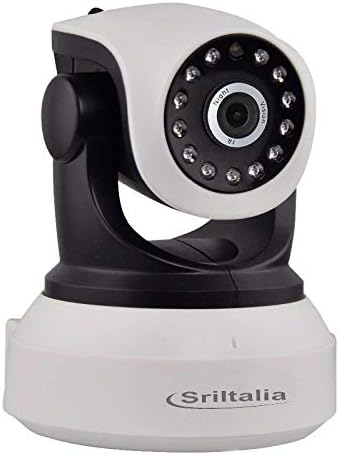
\includegraphics[scale=0.6]{cam.jpg}
    \caption{Sricam SP017}
    \label{fig:sp017}
\end{figure}
\newpage